
\chapter{Background}
\label{chap:background}

This chapter ensures that the reader understands the vocabulary used in this
document. Specifically, this chapter contains the following five parts:

\begin{multicols}{2}
  \begin{enumerate}
  \item \textbf{Graphs}: covers the basic graph types and defines the KG.
  \item \textbf{ML}: describes the three basic ML paradigms as well as some
    activation functions.
  \item \textbf{NLP Techniques}: defined some notions to understand the
    embedding techniques better.
    \columnbreak
  \item \textbf{Attention}: reviews the basics of the attention mechanism
    helpful in understanding the Transformer architecture.
  \item \textbf{Transformer}: introduces the Transformer architecture, used used
    by many recent embedding techniques such as BERT.
  \end{enumerate}
\end{multicols}


\section{Graphs}
\label{sec:background:graphs}

Graphs have been used long before the introduction of ML and cover a wide range
of applications. To better understand the precise vocabulary of graphs, this
section provides some definitions.

\begin{definition}[Graph]
  Ordered pair ($V, E$), where $V$ is a finite and non-empty set of elements
  called \emph{vertices} (or \emph{nodes}), and $E$ is a set of unordered pairs of
  distinct nodes of $V$, called \emph{edges}.
  \label{def:graph}
\end{definition}

\noindent Basic types of graphs include:
\begin{figure}[!ht]
  \begin{minipage}{0.45\linewidth}
    \centering
    \begin{tikzpicture}[minimum size=0.5cm,node distance=1cm]
      \node[entity] (alpha) {1};
      \node[entity,above left=of alpha,xshift=15pt] (beta) {2};
      \node[entity,above right=of alpha,yshift=-5pt,xshift=-5pt] (gamma) {3};
      \node[entity,right=of gamma] (delta) {4};

      \draw[arrow] (alpha) -- (beta);
      \draw[arrow] (beta) -- (gamma);
      \draw[arrow] (alpha) -- (gamma);
      \draw[arrow] (gamma) -- (delta);
    \end{tikzpicture}
  \end{minipage}
  %
  \begin{minipage}{0.5\linewidth}
    \begin{definition}[Oriented Graph]
      Directed Graph where bidirected edges connect no pair of vertices.
      \label{def:oriented:graph}
    \end{definition}
  \end{minipage}
  \vfill
  \vspace{\belowdisplayskip}
  \begin{minipage}{0.45\linewidth}
    \centering
    \begin{tikzpicture}[minimum size=0.5cm,node distance=1cm]
      \node[entity] (alpha) {1};
      \node[entity,above left=of alpha,xshift=15pt] (beta) {2};
      \node[entity,above right=of alpha,yshift=-5pt,xshift=-5pt] (gamma) {3};
      \node[entity,right=of gamma] (delta) {4};

      \draw[arrow] (alpha) -- (beta);
      \draw[arrow] (beta) -- (gamma);
      \draw[arrow] (alpha) -- (gamma);

      \path[arrow] let \p1=($(gamma)-(delta)$),\n1={atan2(\y1,\x1)},\n2={180+\n1} in
      ($ (delta.\n1)!2pt!90:(gamma.\n2) $) edge node {} ($ (gamma.\n2)!2pt!-90:(delta.\n1) $);
      \path[arrow] let \p1=($(delta)-(gamma)$),\n1={atan2(\y1,\x1)},\n2={180+\n1} in
      ($ (gamma.\n1)!2pt!90:(delta.\n2) $) edge node {} ($ (delta.\n2)!2pt!-90:(gamma.\n1)
      $);
    \end{tikzpicture}
  \end{minipage}
  %
  \begin{minipage}{0.5\linewidth}
    \begin{definition}[Directed Graph]
      Named \emph{digraph}, it is defined as a graph whose edges have an
      orientation, also known as \emph{directed edges}, \emph{directed links},
      \emph{arrows}, or \emph{arcs}.
      \label{def:directed:graph}
    \end{definition}
  \end{minipage}
  \caption{Basic Graph Types (Part I).}
\end{figure}

\newpage

\begin{figure}[!ht]
  \begin{minipage}{0.45\linewidth}
    \centering
    \begin{tikzpicture}[minimum size=0.5cm,node distance=1cm]
      \node[entity] (alpha) {1};
      \node[entity,above left=of alpha,xshift=15pt] (beta) {2};
      \node[entity,above right=of alpha,yshift=-5pt,xshift=-5pt] (gamma) {3};
      \node[entity,right=of gamma] (delta) {4};

      \draw (alpha) -- (beta);
      \draw (beta) -- (gamma);
      \draw (alpha) -- (gamma);
      \draw (gamma) -- (delta);
    \end{tikzpicture}
  \end{minipage}
  %
  \begin{minipage}{0.5\linewidth}
    \begin{definition}[Undirected Graph]
      Graph whose edges are bidirectional.
      \label{def:undirected:graph}
    \end{definition}
  \end{minipage}
  \vfill
  \vspace{\belowdisplayskip}
  \begin{minipage}{0.45\linewidth}
    \centering
    \begin{tikzpicture}[minimum size=0.5cm,node distance=1cm]
      \node[entity] (alpha) {1};
      \node[entity,above left=of alpha,xshift=15pt] (beta) {2};
      \node[entity,above right=of alpha,yshift=-5pt,xshift=-5pt] (gamma) {3};
      \node[entity,right=of gamma] (delta) {4};

      \draw[thick] (alpha) -- (beta);
      \draw[thick] (beta) -- (gamma);
      \draw[thick] (alpha) -- (gamma);

      \path[thick] let \p1=($(gamma)-(delta)$),\n1={atan2(\y1,\x1)},\n2={180+\n1} in
      ($ (delta.\n1)!2pt!90:(gamma.\n2) $) edge node {} ($ (gamma.\n2)!2pt!-90:(delta.\n1) $);
      \path[thick] let \p1=($(delta)-(gamma)$),\n1={atan2(\y1,\x1)},\n2={180+\n1} in
      ($ (gamma.\n1)!2pt!90:(delta.\n2) $) edge node {} ($ (delta.\n2)!2pt!-90:(gamma.\n1)
      $);
    \end{tikzpicture}
  \end{minipage}
  %
  \begin{minipage}{0.5\linewidth}
    \begin{definition}[Multigraph]
      Undirected graph that can store multiple edges between two nodes.
      \label{def:multigraph}
    \end{definition}
  \end{minipage}
  \caption{Basic Graph Types (Part II).}
\end{figure}

\noindent Based on these definitions of graph types, the KG is defined.
\begin{definition}[Knowledge Graph]
Directed \emph{heterogeneous} multigraph whose node and relation types have
domain-specific semantics~\citep{website:kamakoti}. These nodes can be of
different types. From a terminology point of view, the nodes/vertices of a KG
are often called \emph{entities}, and the directed edges refer to as
predicates. Moreover, this multigraph has \emph{triple}\footnote{Also called
\emph{triplets}.} designing a 3-tuple, where each triple defines a
(\texttt{subject}, \texttt{predicate}, \texttt{object}) tuple\footnote{Some
authors define this tuple as \texttt{(h, r, t)}. In this definition, \texttt{h}
is the head entity, \texttt{t} the tail entity, and \texttt{r} the relation
associating the head with the tail entities.}. For ease of processing, the
multigraph aspect of the KG can be removed by representing each triple as two
2-tuple: (\texttt{subject} $\rightarrow$ \texttt{predicate}) and
(\texttt{predicate} $\rightarrow$ \texttt{object}).
\end{definition}

%%% Local Variables:
%%% mode: latex
%%% TeX-master: "../../report"
%%% End:


\section{Machine Learning}
\label{sec:background:ml}

Machine Learning (ML) is a branch of AI focusing on improving the automatic
learning of models without having been explicitly programmed for it. ML comes
with three basic paradigms: supervised, unsupervised, and reinforcement
learning. Each of them is defined below.

\begin{multicols}{2}
  \begin{definition}[Supervised Learning]
    Type of ML with human supervision, where a model looks for patterns in a data
    set with labels~\citep{website:deepai:unsupervised:learning}.
    \label{def:supervised:learning}
  \end{definition}

  \begin{definition}[Unsupervised Learning]
    Type of ML with minimal human supervision, where a model looks for patterns
    in a data set without labels.
    \label{def:unsupervised:learning}
  \end{definition}
\end{multicols}

Visually, supervised learning and unsupervised learning are defined as follows:
\begin{figure}[!ht]
  \centering
  \begin{minipage}{.45\textwidth}
    \begin{tikzpicture}[baseline,scale=.7]
      \begin{axis}[
        height=5.5cm,
        width=9cm,
        axis x line=center,
        axis y line=center,
        xlabel style={below right},
        ylabel style={above left},
        xlabel={$X$},
        ylabel={$Y$},
        xtick={4,10},
        xtick={5,14},
        clip mode=individual
        ]

        % Trick to display the graph starting at (1,1)
        \addplot[green,mark size=0] table [%
        x = x,
        y = y,
        col sep = comma]{
          x,y
          0.5,0.5
        };

        \addplot[blue, only marks, mark=*, mark size=3] table [%
        x = x,
        y = y,
        col sep = comma]{
          x,y
          3,3
          3.5,5
          4,4.2
          4.5,3.5
          4.8,2
          5,5
          5.5,4
          6,4.8
          6.5,3.5
        };

        \draw [dashed] (4,11) -- (15,3);

        \addplot[red, only marks, mark=*, mark size=3] table [%
        x = x,
        y = y,
        col sep = comma]{
          x, y
          12,12.5
          12.5,10.5
          13,9
          13.5,11
          14,9.5
          14.5,8
          14.7,12
          14.8,10.7
          15.5,9.6
          16,10.8
        };
      \end{axis}
    \end{tikzpicture}
    \captionof{figure}{Supervised Learning}
    \label{tikz:background:supervised:learning}
  \end{minipage}
  \quad
  \begin{minipage}{.45\textwidth}
    \begin{tikzpicture}[baseline,scale=.7]
      \begin{axis}[
        height=5.5cm,
        width=9cm,
        axis x line=center,
        axis y line=center,
        xlabel style={below right},
        ylabel style={above left},
        xlabel={$X$},
        ylabel={$Y$},
        xtick={4,10},
        xtick={5,14},
        clip mode=individual
        ]

        % Trick to display the graph starting at (1,1)
        \addplot[mark size=0] table [%
        x = x,
        y = y,
        col sep = comma]{
          x,y
          0.5,0.5
        };

        \addplot[black!70,only marks, mark=*, mark size=3] table [%
        x = x,
        y = y,
        col sep = comma]{
          x,y
          3,3
          3.5,5
          4,4.2
          4.5,3.5
          4.8,2
          5,5
          5.5,4
          6,4.8
          6.5,3.5
        };

        \draw [dashed] (5,4) circle[radius=2.8];

        \addplot[black!70,only marks, mark=*, mark size=3] table [%
        x = x,
        y = y,
        col sep = comma]{
          x, y
          12,12.5
          12.5,10.5
          13,9
          13.5,11
          14,9.5
          14.5,8
          14.7,12
          14.8,10.7
          15.5,9.6
          16,10.8
        };
        \draw [dashed] (14.5,10) circle[radius=2.8];
      \end{axis}
    \end{tikzpicture}
    \captionof{figure}{Unsupervised Learning}
    \label{tikz:background:unsupervised:learning}
  \end{minipage}
  \caption{Learning a Model Using Raspberry and Blueberry Data.}
  \label{fig:background:supervised:vs:unsupervised}
\end{figure}

In Figure \ref{tikz:background:supervised:learning}, supervised learning
contains raspberry and blueberry data already classified by their label. A model
learns to predict the values based on a \emph{cost function}, which allows it to
check and correct its predictions according to the actual values. With these
labeled data, the classification and regression problems can use this type of
learning.

In Figure \ref{tikz:background:unsupervised:learning}, unsupervised learning
still contains raspberry and blueberry data. However, this time these data are
not labeled, which means that a model must find the patterns and structure
independently. The clustering and association problems use this type of
learning. For example, this clustering example creates two clusters, with one
raspberry not belonging to any cluster.


\begin{definition}[Reinforcement Learning]
  Type of ML where a model learns from the experience and feedback of an
  autonomous agent.
\end{definition}

\noindent In ML, each neuron inside an Artificial Neural Networks (ANN) outputs
a number between $-\infty$ and $\infty$ propagating to its predecessor via an
activation function. Once the ANN has completed its processing through these
neurons, it generates \emph{logits}, a non-normalized vector of predictions
generated by a classification model. For ease of processing, it is usually
appropriate to convert these logits into probabilities to have a unitary
sum. According to the required type of classification, activation functions such
as \emph{softmax} and \emph{sigmoid} are helpful. These functions can help with
various tasks, such as predicting the most likely word to be the missing word in
a sentence in the Natural Language Processing (NLP) field.

\begin{definition}[Softmax Function]
  Also called \emph{softargmax}, a logistic regression model uses this
  multi-classification function for transformation purposes. Specifically, this
  model transforms a vector of $K$ real values into a vector of $K$ elements that
  range between 0 and 1 with the particularity of having a unitary
  sum~\citep{website:deepai:softmax}. Let $\mathbf{z}$ be an input vector and $K$
  be some classes in a multi-class classifier. Mathematically, the softmax
  function of these classes is defined as follows:
  \begin{equation}
    \mathrm{\sigma}(\mathbf{z})_i = \frac{\me^{z_i}}{\sum^K_{j=1}\me^{z_j}}
    \label{eq:softmax}
  \end{equation}
  \label{def:softmax}
\end{definition}

\begin{definition}[Sigmoid Function]
  Binary classification function recognizable with an ``S'' shaped curve used by
  a logistic regression model for transformation purposes. Unlike the softmax
  function, this model transforms a vector of $K$ real values into a vector of $K$
  elements range this time between -1 and 1 with still the particularity of having
  a unitary sum. Let $\mathbf{x}$ be an input vector. Mathematically, the
  sigmoid function is defined as follows:
  \begin{equation}
    \mathrm{\sigma}(\mathbf{x}) = \frac{1}{1 + e^{-x}} = \frac{e^x}{e^x + 1}
    \label{eq:sigmoid}
  \end{equation}
  \label{def:sigmoid}
\end{definition}

\begin{definition}[Rectified Linear Unit]
  Commonly called \emph{ReLU}, the community considers this function as one of
  the most straightforward functions. Let $\mathbf{x}$ be an input
  vector. Mathematically, the ReLU function is defined as follows:
  \begin{equation}
    \mathrm{f}(\mathbf{x}) = \max(0, \mathbf{x})
    \label{eq:relu}
  \end{equation}
  \label{def:relu}
\end{definition}

\noindent These functions can help with various tasks, such as predicting the
most likely word to be the missing word in a sentence in the NLP
field. Subsequently, in ML, it is essential to know the similarity of two
vectors. For example, it is helpful in NLP to tell if two words share semantic
similarities. As a result, the use of cosine similarity is relevant.

\begin{definition}[Cosine Similarity]
  Measures the cosine of the angle between two non-zero vectors of an inner
  product space~\citep{website:deepai:cosine:similarity}. Let $\mathbf{u},
  \mathbf{v} \in \mathbb{R}^d$ be two non-zero $d$-dimensional vectors.
  Mathematically, the cosine similarity between $\mathbf{u}$ and $\mathbf{v}$ is
  defined as follows:
  \begin{align}
    \cos(\mathbf{u}, \mathbf{v}) =
    \frac{\mathbf{u} \cdot \mathbf{v}}
    {\left\lVert \mathbf{u} \right\rVert
    \left\lVert \mathbf{v} \right\rVert} =
    \frac{\sum\limits_{i = 1}^n u_i v_i}
    {\sqrt{\sum\limits_{i = 1}^n u_i^2}
    \sqrt{\sum\limits_{i = 1}^n v_i^2}}
    \label{eq:cosine:similarity}
  \end{align}

  where $\cos(\mathbf{u}, \mathbf{v})$ produces a value ranging from -1 to 1.
  Specifically, the cosine similarity returns -1 if two vectors do not have any
  similarities, 0 if they are unrelated, and 1 if they share every similarity.
  \label{def:cosine:similarity}
\end{definition}

%%% Local Variables:
%%% mode: latex
%%% TeX-master: "../../report"
%%% End:


\section{Natural Language Processing Techniques}
\label{sec:background:nlp:techniques}

There are many NLP techniques. The objective is not to cover every one of them
but to define certain notions used by more advanced concepts such as Word2Vec.

\begin{definition}[Distributed Representation]
  Describes the same data features across multiple scalable and interdependent
  layers~\citep{website:deepai:distributed:representation}. In a distributed word
  representation, there is a distribution of the word information across vector
  dimensions.
  \label{def:distributed:reprensetation}
\end{definition}

\begin{definition}[Bag-of-Words]
  Vectorizes a text by counting the number of unique words (also called
  \emph{tokens}) in a text. Let ``Suikoden is my favorite game, it is a wonderful
  game!'' be a text. The representation of this text with Bag-of-Words (BoW) is
  defined as follows:
  \begin{equation}
    \left\{\ \text{Suikoden: } 1,\ \text{is: } 2,\ \text{my: } 1,\ \text{favorite: } 1,\
      \text{game: } 2,\ \text{it: } 1, \ \text{a: } 1,\ \text{wonderful: } 1\ \right\}
  \end{equation}

  for which this text can be characterized (e.g., \texttt{[1, 2, 1, 1, 2, 1, 1,
    1]}) by differences measures (e.g., word frequency).
  \label{def:bow}
\end{definition}

\begin{definition}[One-Hot Encoding]
  Quantifies categorical data as binary vectors. Specifically, the belonging of
  a data point to the $i$th category implies the acquisition of a zero value for
  the components of this vector, except for the $i$th component, which receives a
  unitary value.  Let $K$ be several categories in a data set, and
  $\mathbf{y}^{(i)}$ be a data point in the $i$th class. Mathematically, the
  following vectorial representation defines such one-hot encoding:
  \begin{equation}
    \textbf{y}^{(i)} = \underbrace{\begin{bmatrix}0 & \ldots & 0 &
        \underbrace{1}_{\textup{index} \;\; i} &0 & \ldots  &
        0\end{bmatrix}^\top}_{K \times 1}
    \label{eq:one-hot:encoding}
  \end{equation}

  where one-hot encoding vectors allow ML algorithms to make better
  predictions. Such an encoding does not capture words' semantic and syntactic
  information. Therefore, it does not detect semantic and order difference between
  the sentences the ``I like cats more than dogs'' and ``I like dogs more than
  cats'' As a result, \emph{word embeddings} are privileged to detect these
  differences and allow a better numerical representation of words.
  \label{def:one-hot:encoding}
\end{definition}

\begin{definition}[Word Embeddings]
  Unsupervised model that captures words' semantic and syntactic information
  using an \emph{embedding matrix}, where the embeddings of a \textit{w} word are
  a vector $\mathbf{v}_w$.
  \label{def:word:embeddings}
\end{definition}

\begin{definition}[Embedding Matrix]
  Randomized matrix of dimensions $\mathcal{W} \times \mathcal{F}$, where
  $\mathcal{W}$ is the number of unique words in a document and $\mathcal{F}$ is
  the number of features that each unique word in this vocabulary has. The
  \emph{gradient descent} uses these matrix values to find the minima of a
  function for several \emph{epochs}, the number of complete cycles on a training
  data set. From then on, closer words in vector space are assumed to have a
  similar meaning.
  \label{def:embedding:matrix}
\end{definition}

\begin{definition}[Window Size]
  Determines the context words, also called \emph{training samples}, of a target
  word from a sliding window along with a sentence. Therefore, a window size of
  two means 2-triple context words, including the related target word and each of
  the two words on its left and two on its right. Let ``I will always remember
  her'' be a sentence. The following table defines the context words for a window
  size of 2:
  \begin{table}[!ht]
    \centering
    \caption{Context Words Determination for a Window Size of 2. }
    \label{tab:window:size}
    \begin{tabular}{ccc}
      \toprule
      \textbf{Input Text} & \textbf{Target Word} & \textbf{Context Words} \\
      \midrule
      \multirow{2}{*}{\colorbox{blue!25}{I} \colorbox{myblue!25}{will} \colorbox{myblue!25}{always} remember her} & \multirow{2}{*}{i} & will \\
               & & always \\[1.2ex]
      \multirow{3}{*}{\colorbox{myblue!25}{I} \colorbox{blue!25}{will} \colorbox{myblue!25}{always} \colorbox{myblue!25}{remember} her} & \multirow{3}{*}{will} & i \\
                          & & always \\
                          & & remember \\[1.2ex]
      \multirow{4}{*}{\colorbox{myblue!25}{I} \colorbox{myblue!25}{will} \colorbox{blue!25}{always} \colorbox{myblue!25}{remember} \colorbox{myblue!25}{her}} & \multirow{4}{*}{always} & i \\
                          & & will \\
                          & & remember \\
                          & & her \\[1.2ex]
      \multirow{3}{*}{I \colorbox{myblue!25}{will} \colorbox{myblue!25}{always} \colorbox{blue!25}{remember} \colorbox{myblue!25}{her}} & \multirow{3}{*}{remember} & will \\
                          & & always \\
                          & & her \\[1.2ex]
      \multirow{2}{*}{I will \colorbox{myblue!25}{always} \colorbox{myblue!25}{remember} \colorbox{blue!25}{her}} & \multirow{2}{*}{her} & always \\
                          & & remember \\
      \bottomrule
    \end{tabular}
  \end{table}

  In Table \ref{tab:window:size}, the target word highlighted in blue is
  modified at each iteration starting from left to right, considering two words
  forward and backward (highlighted in a lighter blue). As such, the context for a
  given sentence are known.
  \label{def:window:size}
\end{definition}

\begin{definition}[Stop Words]
  Commonly used words (e.g., ``an'', ``the'', and ``is'') having little
  value for training a model and are therefore considered noise in a training
  data set.
  \label{def:stop:words}
\end{definition}

  % \begin{definition}[Mean] Averages of some data. Let $n$ be the data and $\mathbf{x}$ be a
  %   sample. The mean of these data is defined as:
  %   \begin{equation}
  %     \mathrm{\mu} = \frac{1}{n}\sum^n_{i=1}x_i
  %     \label{eq:mean}
  %   \end{equation}
  % \label{def:mean}
  % \end{definition}

  % \begin{definition}[Variance]
  %   Measures how spread a data point is from an average. Let $\mathrm{\mu}$ be the
  %   mean of $n$ data. The variance of a random variable $X$ is defined as:
  %   \begin{equation}
  %     \mathrm{Var}(X) = E\left[\left(X - \mu\right)^2\right]
  %     \label{eq:variance}
  %   \end{equation}
  %   \label{def:variance}
  % \end{definition}

  % \begin{definition}[Standard Deviation]
  %   Measures the dispersion of the data around their center or how they are spread
  %   out in a data set. Let $\mathrm{Var}$ be the variance of $n$ data. The standard
  %   deviation is defined as:
  %   \begin{equation}
  %     \mathrm{\sigma} = \sqrt{\mathrm{Var}(n)}
  %     \label{eq:standard:deviation}
  %     \label{def:standard:deviation}
  %   \end{equation}

  %   where unlike variance, standard deviation is measured using the same units as the data.
  % \end{definition}

%%% Local Variables:
%%% mode: latex
%%% TeX-master: "../../report"
%%% End:


\section{Attention}
\label{sec:attention}

The \emph{Attention} is a Deep Learning mechanism published in 2014 by
\textsc{Bahdanau} et al. to solve the bottleneck issue of Recurrent Neural
Networks (RNNs) sequential models widely used for neural machine
translation~\citep{bahdanau}. To fully understand its mechanism, it is helpful
to start by introducing the functioning of RNNs.

\subsection{Recurrent Neural Networks}
\label{subsec:rnns}

Before using such a mechanism, RNNs caused accuracy losses for a model when
processing long input sequences mainly due to the way RNN encoders generated the
context vector. Added to that, RNNs are difficult to parallelize.

\begin{figure}[!ht]
  \centering
  \begin{tikzpicture}[
    hid/.style 2 args={rectangle split, rectangle split horizontal, draw=#2,
      rectangle split parts=#1, fill=#2!20, outer sep=1mm},
    label/.style={font=\small}]
    \tikzset{>=stealth',every on chain/.append style={join},
      every join/.style={->}}

    \foreach \step in {1,2,3,4,5,6,7} {
      \node[hid={3}{blue}] (w\step) at (2.5*\step, -1.5) {};
      \node[hid={3}{red}] (o\step) at (2.5*\step, 1.5) {};
      \node[label,rectangle, draw=grey, fill=grey!20,
     minimum height=0.22cm,minimum width=1.4cm] (h\step) at (2.5*\step, 0) {\scriptsize{RNN}};
      \draw[->] (w\step.north) -> (h\step.south);
      \draw[->] (h\step.north) -> (o\step.south);
    }

    \foreach \step/\next in {1/2,2/3,3/4,4/5,5/6,6/7}
    \draw[->] (h\step.east) -> (h\next.west) node[above,midway] {$h_\step$};

    \node[label,below=of w1,yshift=30pt] {hello};
    \node[label,below=of w2,yshift=28pt] {my};
    \node[label,below=of w3,yshift=30pt] {dear};
    \node[label,below=of w4,yshift=28pt] {\texttt{<EOS>}};
    \node[label,below=of w5,yshift=30pt] {bonjour};
    \node[label,below=of w6,yshift=28pt] {ma};
    \node[label,below=of w7,yshift=30pt] {chère};

    \node[label,above=of h1.north,yshift=13pt] {$o_1$};
    \node[label,above=of h2.north,yshift=13pt] {$o_2$};
    \node[label,above=of h3.north,yshift=13pt] {$o_3$};
    \node[label,above=of h4.north,yshift=13pt] {bonjour};
    \node[label,above=of h5.north,yshift=15pt] {ma};
    \node[label,above=of h6.north,yshift=15pt] {chère};
    \node[label,above=of h7.north,yshift=15pt] {\texttt{<EOS>}};

    \draw[loosely dashed, thick] (8.75,3) -- (8.75,1);
    \draw[loosely dashed, thick] (8.75,-0.5) -- (8.75,-2.5);

    \node[label,above=of h2.north,yshift=35pt] {\textbf{ENCODER}};
    \node[label,above=of h5.north,yshift=35pt,xshift=30pt] {\textbf{DECODER}};
  \end{tikzpicture}
  \caption{Sequence-to-Sequence Learning With RNNs.}
  \label{fig:rnn}
\end{figure}

In Figure \ref{fig:rnn}, a Sequence to Sequence (Seq2Seq) model translates an
English sentence into French using RNN encoders and decoders. Each time step has
an RNN unit containing an activation function that takes a word embedding and a
hidden state as input for both encoding and decoding. This hidden state serves
as a memory to save the entire previous context. Specifically, the hidden state
at the $t$ time step is computed based on the hidden state at the $t − 1$ time
step and the current word embedding. Once one RNN encoder reaches the first
End-Of-Sentence (\texttt{<EOS>}), the RNN decoder receives a context vector
containing the last generated hidden state, namely $h_3$. Finally, each RNN
decoder unit translates a word based on this context until to reach once more
the \texttt{<EOS>} token.

Although RNNs are effective for small sequences, this is not the case for more
extensive sequences. This mechanism uses a fixed size context vector and
generates the encoder's hidden states based on the previous hidden
state. Consequently, the last words of an input sequence have a greater weight
than the first ones. From this unbalanced weight, processing a long sequence by
a model comes at the cost of forgetting the earlier parts of that sequence,
resulting in a loss model's accuracy. RNN variants emerged to reduce this waste
of information, such as Long Short-Term Memory (LSTM) and Gated Recurrent Units
(GRU). These variants helped to improve the model's accuracy, but the Attention
mechanism came up with an interesting idea.

\subsection{Mechanism}
\label{subsec:attention:mechanism}

The basic idea of the Attention mechanism is not only to pay attention to each
input word in the context vector but also to give a relative importance to each
of them~\citep{bahdanau}. In other words, the Attention mechanism focuses on
matching input and output elements. After its publication, this mechanism became
one of the design choices in many NLP and Computer Vision tasks. Computer Vision
is a field of Artificial Intelligence where the computer learns digital images
or video content. This mechanism has received other
variants~\citep{DBLP:conf/emnlp/LuongPM15}, which increased the model's accuracy
in most of the benchmarks that have been performed. Finally, due to the
popularity of the Attention mechanism, the use of RNNs has been questioned many
times. However, RNNs are still present in everyday life through various voice
assistance applications such as Apple's Siri, Amazon Alexa, and Google Home.

With the Attention mechanism, the context vector includes each encoder's hidden
state. In addition, each decoder's hidden state processes some additional
calculation to achieve a better model's accuracy compared to the use of RNNs
without Attention~\citep{alammar-seq2seq}. This mechanism mainly solved the
previous issues related to the lack of parallelization and forgetting previous
word contexts for long sequences.


\newpage

Visually, the mechanism works as follows:
\begin{figure}[!ht]
  \centering
  \begin{tikzpicture}[
    hid/.style 2 args={rectangle split, rectangle split horizontal, draw=#2,
      rectangle split parts=#1, fill=#2!20, outer sep=1mm},
    label/.style={font=\small}]
    \tikzset{>=stealth',every on chain/.append style={join},
      every join/.style={->}}

    \foreach \step in {1,2,3} {
      \node[label,rectangle, draw=grey, fill=grey!20,
      minimum height=0.22cm,minimum width=1.35cm] (w\step) at (2.5*\step, -1.5) {\scriptsize{RNN}};
      \node[hid={3}{blue},below=of w\step,yshift=20pt] (e\step) {};
      \draw[->] (e\step) -> (w\step);
    }


     \node[label,rectangle, draw=grey, fill=grey!20,
      minimum height=0.22cm,minimum width=1.35cm] (w4) at (12.25,-1.5) {\scriptsize{RNN}};
     \node[label,rectangle, draw=grey, fill=grey!20,
     minimum height=0.22cm,minimum width=1.35cm] (w5) at (14.75,-1.5) {\scriptsize{RNN}};

     \node[right=of w5,xshift=-20pt] (dots) {$\dotso$};

    \node[hid={3}{blue},below=of w4,yshift=20pt] (e4) {};
    \node[hid={3}{red},below=of w5,yshift=20pt,opacity=0.4] (e5) {};
    \draw[->] (e4) -> (w4);
    \draw[->] (e5) -> (w5);

    \foreach \step/\next in {1/2,2/3}
    \draw[->] (w\step.east) -> (w\next.west) node[above,midway] (h\step) {$h_\step$};

    \draw[->] (w3.east) -> ([xshift=30pt]w3.east) node[above,midway] (h3) {$h_3$};
    \draw[->] ([xshift=-50pt]w4.west) -> (w4.west) node[above,midway] (c) {$h_1,h_2,h_3$};
    \draw[->] (w4) -> (w5) node[above,midway] (h4) {$h_4$};

    \foreach \step in {1,2,3}{
    \node[circle,fill=green!20,draw=green,outer sep=1mm,minimum
    size=0.8cm,scale=0.8,above=of h\step] (dot\step) {.};
    \draw[->] (h\step.north) -> (dot\step.south);
    }

    \node[circle,fill=red!30,draw=red,outer sep=0.1mm,above=of dot1,minimum size=0.8cm,scale=0.85] (s1) {\scriptsize{$9.7$}};
    \node[circle,fill=red!20,draw=red,outer sep=0.1mm,above=of dot2,minimum size=0.8cm,scale=0.85] (s2) {\scriptsize{$2.1$}};
    \node[circle,fill=red!10,draw=red,outer sep=0.1mm,above=of dot3,minimum size=0.8cm,scale=0.85] (s3) {\scriptsize{$1.2$}};

    \node[rectangle,draw,above=of s1,minimum width=6cm,minimum height=1cm,xshift=72.5pt] (r) {};
    \node[rectangle,draw=mygreen,above=of s1,fill=mygreen,minimum height=0.7cm,yshift=0.9pt] (r1) {};
    \node[rectangle,draw=mygreen,above=of s2,fill=mygreen,minimum height=0.2cm,yshift=0.9pt] (r2) {};
    \node[rectangle,draw=mygreen,above=of s3,fill=mygreen,minimum height=0.1cm,yshift=0.9pt] (r3) {};

    \node[label,below=of e1,yshift=30pt] {hello};
    \node[label,below=of e2,yshift=28pt] (my) {my};
    \node[label,below=of e3,yshift=30pt] {dear};
    \node[label,below=of e4,yshift=28pt] (eos) {\texttt{<EOS>}};
    \node[label,below=of e5,yshift=30pt,opacity=0.7] (bonjour) {bonjour};

    \draw[arrow] ([xshift=-20pt]dot3.west) |- (dot2.east);
    \draw[arrow] ([xshift=-20pt]dot2.west) |- (dot1.east);

    \draw ([xshift=-20pt]dot3.west) |- ([xshift=-20pt,yshift=-25pt]dot3.west);
    \draw ([xshift=-20pt]dot2.west) |- ([xshift=-20pt,yshift=-30pt]dot2.west);

    \draw[arrow] ([xshift=5pt]h4.north) |- (dot3.east);
    \draw (h4) |- ([xshift=-20pt,yshift=-25pt]dot3.west);
    \draw ([xshift=-10pt]h4) |- ([xshift=-20pt,yshift=-30pt]dot2.west);

    \foreach \step in {1,2,3}
    \draw[arrow] (dot\step) -- ([yshift=-2pt]s\step);

    \foreach \step in {1,2,3}
    \draw[arrow] (s\step) -- ([yshift=-2pt]r\step.south);

    \node[circle,above=of r1.south,yshift=10pt,fill=green!20,draw=green,outer sep=1mm,minimum size=0.8cm,scale=0.8] (mul1) {x};
    \node[circle,above=of r2.south,yshift=30pt,fill=green!20,draw=green,outer sep=1mm,minimum size=0.8cm,scale=0.8] (mul2) {x};
    \node[circle,above=of r3.south,yshift=50pt,fill=green!20,draw=green,outer sep=1mm,minimum size=0.8cm,scale=0.8] (mul3) {x};

    \node[hid={3}{blue},above=of mul1,yshift=28pt] (W1) {};
    \node[hid={3}{blue},above=of mul2,yshift=8pt] (W2) {};
    \node[hid={3}{blue},above=of mul3,yshift=-10pt] (W3) {};

    \node[label,above=of W1,yshift=-30pt] {hello};
    \node[label,above=of W2,yshift=-32pt] {my};
    \node[label,above=of W3,yshift=-30pt] {dear};

    \foreach \step in {1,2,3}
    \draw[arrow] (W\step) -- (mul\step);

    \draw[arrow] ([xshift=-2.535cm]r.north) -| (mul1.south);
    \draw[arrow] ([xshift=-0.05cm]r.north) -| (mul2.south);
    \draw[arrow] ([xshift=2.4cm]r.north) -| (mul3.south);

    \node[circle,right=of mul2.east,xshift=70pt,fill=green!20,draw=green,outer
    sep=1mm,minimum size=0.8cm,scale=0.8] (sum) {+};

    \node[hid={3}{red},right=of sum] (output) {};
    \node[label,above=of output,yshift=-30pt] (output_label) {bonjour};
    \draw[arrow] (sum) -- (output);

    \draw[arrow] (mul1.east) -| (sum.south);
    \draw[arrow] (mul2.east) -- (sum);
    \draw[arrow] (mul3.east) -| (sum.north);

    \node[label,left=of dot1, xshift=0.5cm] {Dot Product};
    \node[label,left=of s1, xshift=0.45cm] {Attention Score};
    \node[label,left=of r1, xshift=0.35cm] {Attention Weights};
    \node[label,left=of mul1,yshift=20pt,xshift=0.55cm] {Weighted Sum};

    \node[label,below=of my.south,yshift=23pt] {\textbf{ENCODER}};
    \node[label,below=of eos.south,yshift=25pt] {\textbf{DECODER}};

    \node[right=of dot1,xshift=-30pt,yshift=7pt] {\footnotesize{query}};
    \node[right=of dot2,xshift=-30pt,yshift=7pt] {\footnotesize{query}};
    \node[right=of dot3,xshift=20pt,yshift=7pt] {\footnotesize{query}};

    \node[above=of h1,xshift=-12pt,yshift=-15pt] {\footnotesize{key}};
    \node[above=of h2,xshift=-12pt,yshift=-15pt] {\footnotesize{key}};
    \node[above=of h3,xshift=-12pt,yshift=-15pt] {\footnotesize{key}};

    \node[right=of mul1,xshift=-25pt,yshift=7pt] {\footnotesize{value}};
    \node[right=of mul2,xshift=-25pt,yshift=7pt] {\footnotesize{value}};
    \node[right=of mul3,xshift=-25pt,yshift=7pt] {\footnotesize{value}};
  \end{tikzpicture}
  \caption{Seq2Seq Learning With Attention Mechanism.}
  \label{fig:attention}
\end{figure}

In Figure \ref{fig:attention}, the Attention mechanism starts using the encoder
RNNs to generate their hidden states, similar to Figure \ref{fig:rnn}. Once
these hidden states have been generated, the context including these hidden
states is provided to each time step of the decoder RNNs. For each RNN decoder
block, the hidden state of decoding is calculated in three significant steps:
\begin{enumerate}
\item \textbf{Computation of the Attention/Alignment Score for each word}: to
  know the most likely word to pay more attention to the translation of the
  current word, a dot product is made between the previous decoding hidden state
  with every encoding hidden state.

  The original research paper defines \emph{query}, \emph{key}, and \emph{value}
  by making an analogy with a database. The query allows performing a search
  (e.g., book) associated with a set of keys (e.g., book title and abstract) for
  which each key is associated with a value. From then on, the \emph{Dot-Product
    Attention} consists of computing the weighted matching between $m$ queries and
  $n$ keys in an $m$ by $n$ matrix.

\item \textbf{Computation of the Attention Weights}: the Attention scores are
  normalized with a softmax function in such a way as to ease their processing
  using a probability distribution whose sum is unitary.
  \begin{definition}[Attention Score]
    Let $h_1, \ldots, h_N \in \mathbb{R}^h$ be encoder hidden states, $s_t \in
    \mathbb{R}^h$ be the decoder hidden state, and $t$ be the time
    step. Mathematically, the $\mathrm{a}_t$ Attention score is defined as follows:
    \begin{align}
      \alpha^t &= \mathrm{softmax}\left(\left[  s_t^Th_1, \ldots, s_t^Th_N \right]\right) \in \mathbb{R}^N \\
      \mathrm{a}_t &= \sum^N_{i=1}\alpha^t_ih_i \in \mathbb{R}^N
      \label{eq:def:attention:score}
    \end{align}
    \label{def:attention:score}
  \end{definition}

\item \textbf{Computation of the weighted sum}: After normalization, it is
necessary to multiply each embedded word with its weight to compute the hidden
state.
\end{enumerate}

After the calculation of the hidden states, Attention picks the most likely word
for translation. This mechanism gives importance to these words by mapping them
to a higher or lower weight depending on the word’s relevance. Therefore, this
improves the accuracy of the output predictions~\citep{bahdanau}. However, the
Attention mechanism in Figure \ref{fig:attention} cannot be used in a neural
network since there are no weights to train by a model. In practice, the
Attention mechanism uses three weight matrices to multiply each key, value, and
query by their respective matrices called the key, query, and value matrices.

Following the publication of Attention, another attention mechanism emerged
which gives attention within input elements. \emph{Self-Attention} also called
\emph{intra-attention}, is a Attention mechanism defines in 2016 and relates
different positions of a single sequence to compute a representation of the same
sequence~\citep{Cheng}. Unlike the primary Attention mechanism, where the query,
key, and value matrices may differ, Self-Attention has these three matrices
identically as generated from the same input sequence. Based on a gradient
signal, each self-attention block can use this signal to propagate information
to the weight matrices, namely the key, query, and values matrices. It is
largely thanks to Self-Attention that the \emph{Transformer} architecture was
created.

%%% Local Variables:
%%% mode: latex
%%% TeX-master: "../../report"
%%% End:


\section{Transformer}
\label{sec:transformer}

The \emph{Transformer} architecture is an alternative to RNNs published in 2017,
questioning the need for RNNs following the discovery of the Attention
mechanism~\citep{vaswani:attention}. The original paper presents this
architecture for Machine Translation and introduces two new Attention
mechanisms: \emph{Scaled Dot-Product Attention} and \emph{Multi-Head Attention}.

\subsection{Scaled Dot-Product Attention}
\label{subsec:transformer:scaled:dot-prodct:attention}

\emph{Scaled Dot-Product Attention} provides an Attention score based on a Dot
Product Attention scaled by the square root inverse of the dimension of the
query and key matrices. This scaled version prevents the Dot-Product Attention
mechanism from growing large in magnitude when the dimensionality of the queries
has a high value. Specifically, this high value is due to the multiplication and
the addition of inputs, which push the softmax function into regions where its
gradients are minimal.
\begin{definition}[Scaled Dot-Product Attention]
  Let $Q \in \mathbb{R}^{m\times d_k}$ be the matrix of queries and $K \in
  \mathbb{R}^{n\times d_k}, V \in \mathbb{R}^{m\times d_v}$ be matrices of a set
  of key-value pairs. Mathematically, the the Scaled Dot-Product Attention
  mechanism is defined as follows:
  \begin{equation}
    \mathrm{A}(Q, K, V) = \mathrm{softmax}\left(\frac{QK^T}{\sqrt{d_k}}\right)V
    \label{eq:def:scaled:dot-product:attention}
  \end{equation}

  where $d_k$ is the dimensionality of queries as well as keys and $d_v$ the
  dimensionality of values.
\end{definition}

\subsection{Multi-Head Attention}
\label{subsec:transformer:multi-head:attention}

\emph{Multi-Head Attention} (MHA) is an improved version of the Self-Attention
mechanism where each word not only brings excessive importance to itself, but
pays attention to the interactions with other words. As a result, MHA achieves
better results than Self-Attention, where the latter leads to a loss of
efficiency in the Attention embeddings. Finally, MHA still performs a weighted
average to generate the Attention vector for each token. However, the heads are
this time computed in parallel.

\begin{definition}[Multi-Head Attention]
  Let $f_o: \mathbb{R}^{kd} \to \mathbb{R}^D$ be a linear map, $f_{i,q}, f_{i,
    k}, f_{i, v}: \mathbb{R}^D \to \mathbb{R}^d$ be a three sets of linear maps,
  $\hat{Q} \in \mathbb{R}^{M\times D}$ be a queries vector, and $\hat{K}, \hat{V}
  \in \mathbb{R}^{N\times D}$ be vectors of keys and values. Mathematically, the
  MHA is defined as follows:
  \[
    \textrm{MHA}(\hat{Q}, \hat{K}, \hat{V}) = f_o \left (
      \text{concat} \left (
        \left [
          A \left (
            f_{i,q}(\hat{Q}),
            f_{i,k}(\hat{K}),
            f_{i,v}(\hat{V})
          \right )
          \
          \forall \ i \in 1,\dots, k
        \right ]
      \right )
    \right )
  \]
  where $\text{MHA}(\hat{Q}, \hat{K}, \hat{V}) \in \mathbb{R}^{M \times D}$ is
  the output of the MHA, also known as a \emph{neural function} with $k$-headed
  attention block.
\end{definition}

\subsection{Architecture}
\label{subsec:transformer:architecture}

The Transformer architecture mainly consists of an encoder and a decoder block,
including the Scaled Dot-Product and MHA mechanisms. Specifically, the encoder
and decoder are neural components composed of a stack of $N=6$ identical layers.

Visually, one layer of the Transformer works as follows:
\begin{figure}[!ht]
  \centering
  \subfloat[Encoder\label{fig:transformer:encoder}]{%
    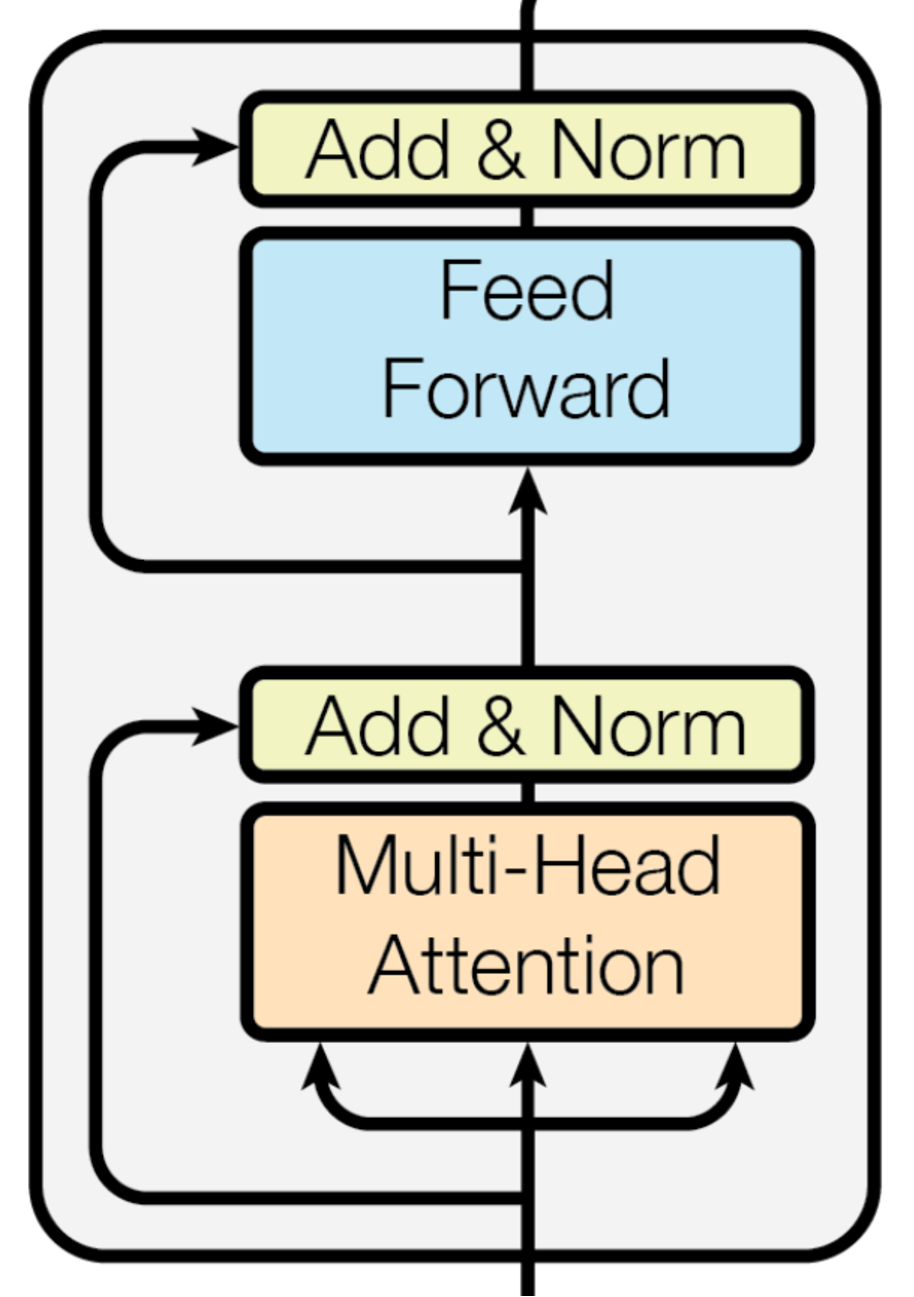
\includegraphics[width=0.23\textwidth]{img/transformer/encoder}
  }
  \quad
  \subfloat[Decoder\label{fig:transformer:decoder}]{%
    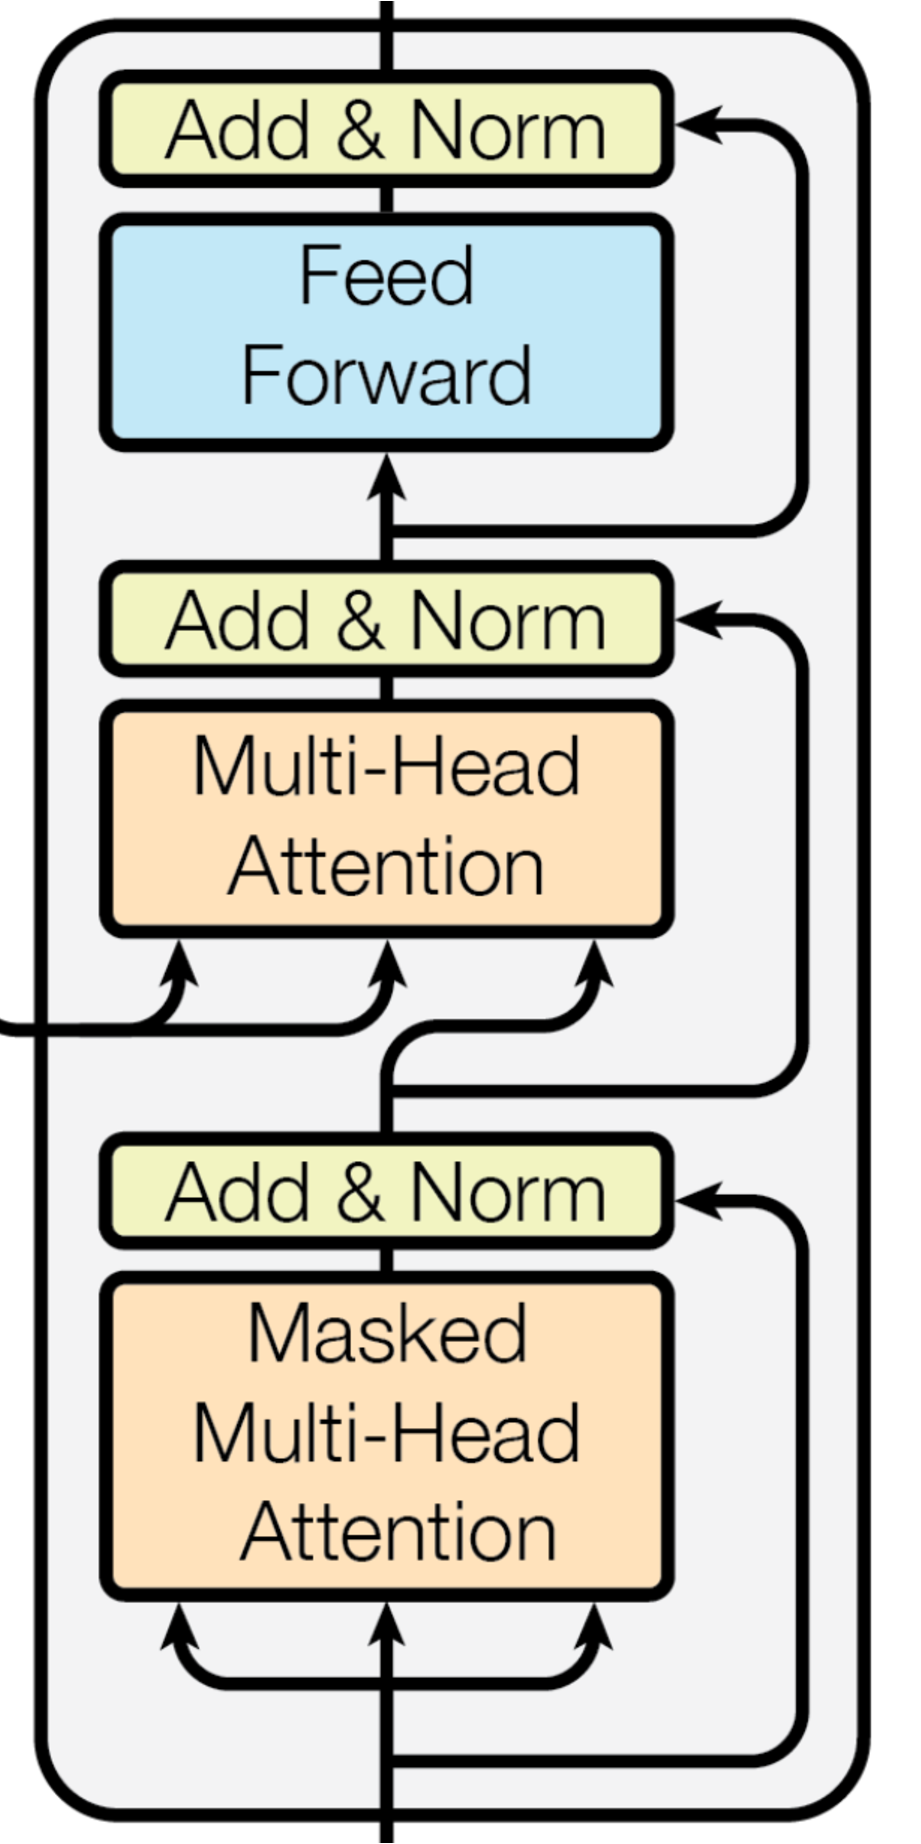
\includegraphics[width=0.23\textwidth]{img/transformer/decoder}
  }
  \caption{One Layer of the Architecture of the Transformer.}
  \label{fig:transformer:architecture:encoder}
  \source{\textsc{Vaswani} et al. -- Attention Is All You Need.}
\end{figure}

In Figure \ref{fig:transformer:encoder}, one layer of the encoder contains two
sub-layers: a MHA mechanism and a position-wise fully connected Feed-Forward
Neural Network (FFN).
\begin{definition}[Feed-Forward Neural Network]
  Let $W_1 + b_1$ and $W_2 + b_2$ be two linear transformations. Mathematically,
  the FFN is defined as follows:
  \begin{equation}
    \mathrm{FFN}(x) = \max\left(0, xW_1 + b_1\right)W_2 + b_2
    \label{eq:def:ffn}
  \end{equation}
  where a ReLU activation function is used.
  \label{def:ffn}
\end{definition}

Moreover, a residual connection followed by a normalization of the layers wraps
each of the two sublayers. Mathematically, the output of every sub-layer is
defined as follows:
\begin{equation}
  \mathrm{LayerNorm}(x + \mathrm{Sublayer}(x))
  \label{eq:output:sub-layer}
\end{equation}
where $\mathrm{Sublayer}(x)$ refers to the implemented function by the sub-layer
itself. \\


\noindent In Figure \ref{fig:transformer:decoder}, the decoder has layers that
differ from the encoder with two sub-layer changes. The first sublayer change is
defined using \emph{Masked MHA} as the first sub-layer to prevent positions from
attending subsequent positions. The last change is adding a new sub-layer,
called \emph{Encoder-Decoder Attention} which performs MHA over the Attention
vectors of the decoder and those of the encoder. The use of this sub-layer makes
it possible to determine the different relationships between these
vectors. Finally, the generated embeddings are sent to a position-wise fully
connected FFN. Like the encoder, each sub-layer is wrapped by a residual
connection followed by a layer normalization.

From then one, the complete architecture of the Transformer is illustrated as follows:
\begin{figure}[!ht]
  \centering
  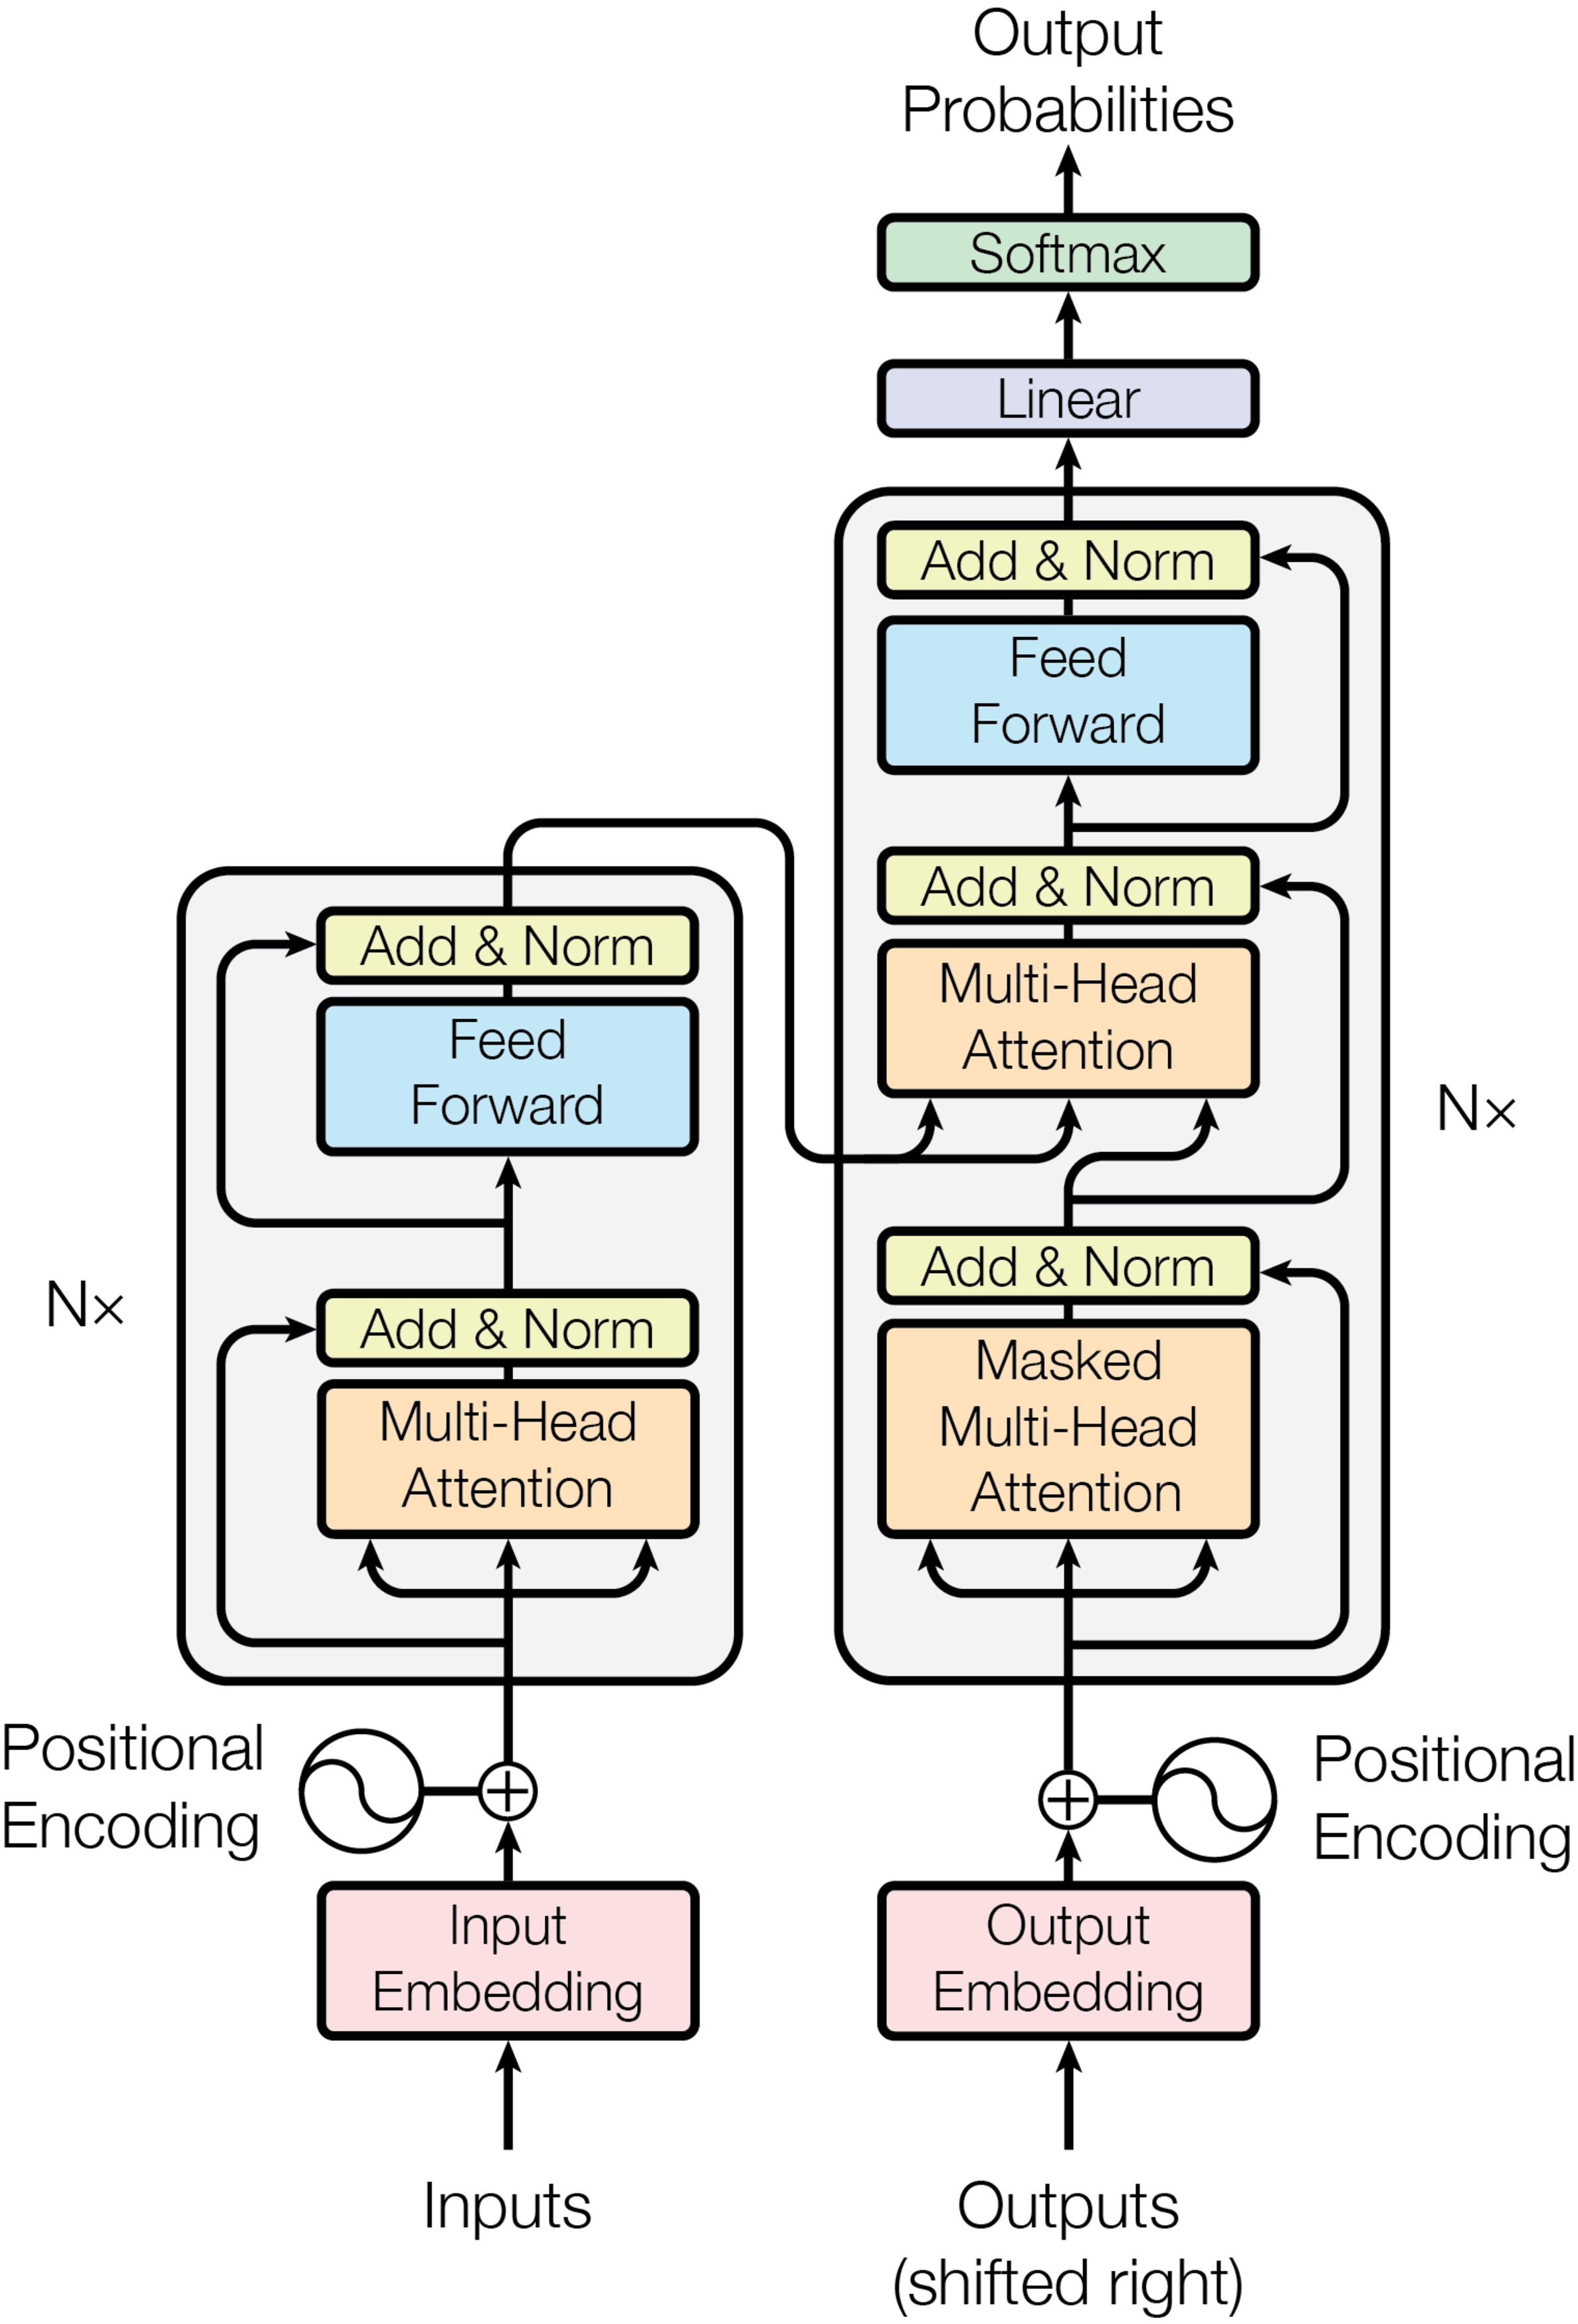
\includegraphics[width=0.6\textwidth]{img/transformer/architecture}
  \caption{Model Architecture of the Transformer.}
  \source{\textsc{Vaswani} et al. -- Attention Is All You Need}
  \label{fig:transformer:architecture}
\end{figure}

\newpage

In Figure \ref{fig:transformer:architecture}, both encoding and decoding take
the sum of the input/output embeddings with positional embedding as
input. Unlike RNNs, Transformer do not have a time step so that input sequences
can be injected simultaneously and converted into input embeddings. Each token
is represented in the embedding space through these input embeddings where
semantically similar tokens are closer than others. However, the decoder has the
particularity of having its input shifted. This shift avoids that a model only
learns to copy the decoder input by allowing a model to predict the target
word/character for position $i$ according to the previous one from 1 to $i-1$.

At last, the output of the decoding layer is sent to a linear layer. This layer
is nothing more than an FFN layer whose objective is to extend the dimension of
this vector to the number of words of the language concerned. Once expanded,
this vector is submitted to a softmax activation function to transform it into a
probability distribution and predict the next word according to the word with
the highest probability. Afterward, this decoding process is iterated several
times until the end-of-sentence token is generated.

\subsection{Positional Encoding}
\label{subsec:transformer:positional:encoding}

Considering that the transformer has no recurrence or convolution mechanism, the
architecture cannot know the order in an input sequence. From then on, the
transformer encodes the same meaning for different sentences. The easiest way to
take this context into account is to encode these positions as one-hot features.
\begin{definition}[Positional Encoding as One-Hot Features]
  Let $x \in \mathbb{R}^{n \times d}$ be a matrice of sequentially ordered data
  along the $n$-dimensional axis, and $e_k$ be a $k$'th standard basis vector in
  $\mathbb{R}^n$. Mathematically, the $z \in \mathbb{R}^{n \times d}$ learned
  combined representation is defined as follows:
  \begin{equation}
    \mathrm{z}_k = W^T_zReLU\left(W_x^Tx_k + W_e^Te_k\right), W_x \in
    \mathbb{R}^{dim(x)\times m}, W_e \in \mathbb{R}^{n\times m}, W_z \in \mathbb{R}^{m\times d}
    \label{eq:def:positional:encoding:one:hot}
  \end{equation}
  \label{def:positional:encoding:one:hot}
\end{definition}

\noindent Another approach for positional encoding is to build distinct
representations of inputs and positions~\citep{gehring}. Despite these existing
approaches to differentiate meanings, the original Transformer paper uses a
sinusoid-wave-based positional encoding to inject absolute positional
information of tokens into the sequence.

\begin{definition}[Positional Encoding by \textsc{Vaswani} et al.]
  Let $d_{model}$ be the embedding dimension of words, and $pos \in \left[0, L -
    1\right]$ be the position of a $w$ word in the $w = (w_0,\dotsc,w_{L-1})$ input
  sequence. Mathematically, the positional encoding of $w$ is defined as follows:
  \begin{align}
    \mathrm{PE}(pos,i) = \begin{cases}
      \sin\displaystyle\left(\frac{pos}{10000^{2i/d_{model}}}\right)\,, & i = 2k \\\\
      \cos\displaystyle{\left(\frac{pos}{10000^{2i/d_{model}}}\right)}\,, & i = 2k + 1
    \end{cases} \   k \in \mathbb{N}
    \label{eq:positional:encoding}
  \end{align}

  where the positional encoding follows a specific, learned pattern to identify
  word position or the distance between words in the sequence~\citep{alammar}.  In
  Equation \ref{eq:positional:encoding}, the sinusoidal representation works as
  well as a learned representation and better generalizes sequences that are
  longer than the training sequences~\citep{vaswani:attention}.
\end{definition}

%%% Local Variables:
%%% mode: latex
%%% TeX-master: "../../report"
%%% End:


%%% Local Variables:
%%% mode: latex
%%% TeX-master: "../report"
%%% End:
